Der Ursprung der Web Graphics Library liegt in der Arbeit des inzwischen bei Mozilla angestellten Software-Entwicklers Vladimir Vukićević. Dieser präsentierte 2006 einen ersten experimentellen Prototypen einer Schnittstelle des HTML5-Canvas-Elements\footnote{Canvas: engl. für \enquote{Leinwand}.} zur Grafikbibliothek OpenGL \autocite{WEBGL_ORIGIN_VUKICEVIC}.
Dieser neue Ansatz sollte die native Darstellung von 3D-Grafik im Webbrowser ermöglichen. Hierin liegt der fundamentale Unterschied und Vorteil WebGLs gegenüber allen vorherigen Web3D-Ansätzen: Durch die direkt in den Browser integrierte Schnittstelle zu OpenGL sind Plugins für die Berechnung von 3D-Grafik nicht länger notwendig.

Sowohl Firefox als auch Opera realisierten ein Jahr nach Vukićevićs Vorstoß frühe, eigenständige Implementierungen dieses Ansatzes innerhalb ihrer Browser \autocite{WEBGL_ORIGIN_VUKICEVIC} \autocite{WEBGL_ORIGIN_OPERA}. Während Mozillas Umsetzung von Canvas-3D eine nahezu direktes \emph{Mapping} von JavaScript zu OpenGL darstellte, war Operas Ansatz etwas abstrahierter, um eine bessere Plattformunterstützung zu erzielen.

Zur Standardisierung dieses neuen Vorstoßes für 3D-""Grafik im Web bildete sich 2009 daraufhin die WebGL-Arbeitsgruppe innerhalb der \textit{Khronos Group}. Zwei Jahre später wurde Version 1.0 der Spezifikation auf Basis von \emph{OpenGL ES 2.0} im Februar 2011 fertig gestellt \autocite{KHRONOS_WEBGL_SPEC_10}. Die Khronos Group ist ein seit 2000 bestehendes internationales Industriekonsortium, welches die Entwicklung zahlreicher lizenzfreier und offener Standards im Multimedia-Bereich vorantreibt \autocite{KHRONOS_GROUP_ABOUT}. Zahlreiche namhafte Organisationen und IT-Unternehmen wie Apple, Google, Mozilla und Opera beteiligen sich seither aktiv bei der Entwicklung von WebGL \autocite{KHRONOS_GROUP_WEBGL}.

\subsection{Grundarchitektur}

% TODO: ZEILENNUMMERN ÜBERPRÜFEN!!!

Um die grundlegende Architektur einer WebGL basierten Webanwendung zu verstehen, werden zu Anfang die beteiligten Technologien und deren Zusammenspiel erörtert. Die schematische Abbildung \ref{FIG:WEBGL_ARCHITECTURE} veranschaulicht die Beziehung der einzelnen Komponenten untereinander:

\begin{figure}[ht]
	\centering
	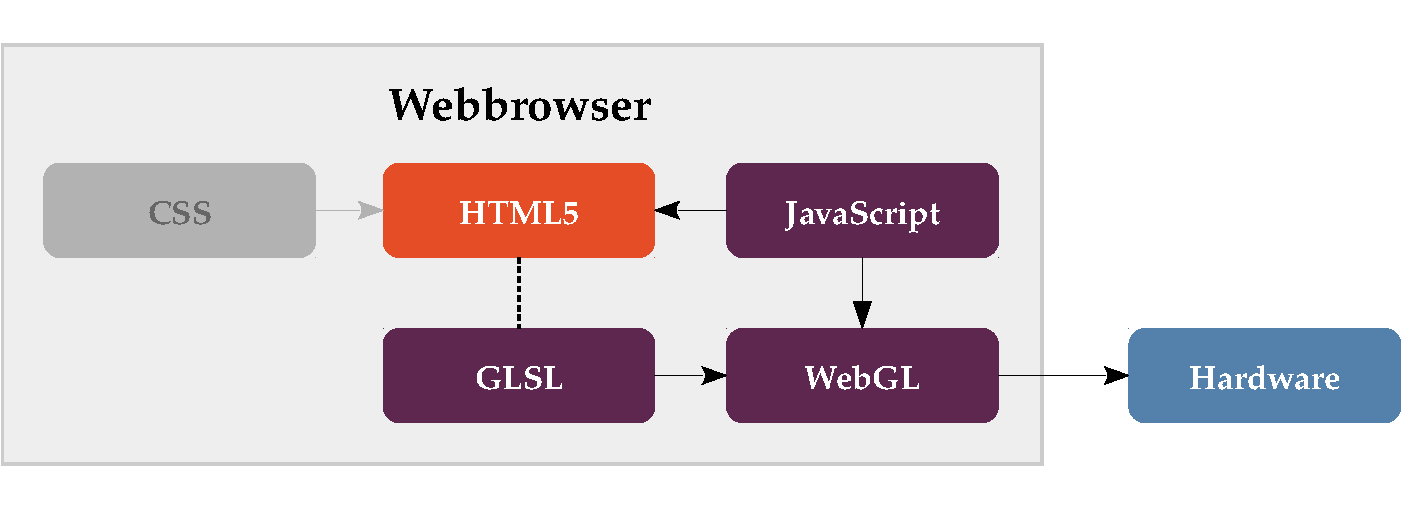
\includegraphics[width=0.8\textwidth]{kap4/webgl/figures/architecture-crop.pdf}
	\caption{Grundarchitektur einer WebGL-basierten Web3D-Anwendung.}
	\label{FIG:WEBGL_ARCHITECTURE}
\end{figure}

Zur Darstellung der 3D-""Grafik ist zunächst ein konventionelles HTML-Dokument nötig. Wichtig ist hierbei eine Deklaration des Dokumentyps als HTML5, da WebGL das erst mit HTML5 eingeführte Canvas-Element benötigt.
Obgleich dieser neue Standard derzeit noch nicht den höchsten Reifegrad einer \emph{W3C Recommendation} erlangt hat, ist dessen Entwicklung weit vorangeschritten. So wurde bereits im Mai 2011 der \enquote{\emph{Last Call}} ausgerufen, also die Aufforderung, letzte Änderungensvorschläge für den Entwurf einzureichen \autocite{W3C_HTML5_LAST_CALL_TARGET_2014}. Weiterhin wurde in selbiger Ankündigung das Jahr 2014 als Zeitpunkt für den Statuswechsel der Spezifikation zu einer W3C-Empfehlung anvisiert.

Das Canvas-Element stellt eine rechteckige Zeichenfläche dar, welche durch JavaScript angesteuert wird und der dynamischen Generierung von Grafiken dient \autocite{W3C_HTML5_SPEC_WORKING_DRAFT}.
Das Element verfügt über mehrere sogenannte \emph{Kontexte}. Ein Kontext stellt die Schnittstelle zu einer Grafik-Implementierung dar und erlaubt es, JavaScript auf der Leinwand zu zeichen. Während der Kontext mit der Bezeichnung \texttt{2d} zweidimensionale Grafiken ermöglicht, kann das Element ebenso als Projektionsfläche dreidimensionaler Grafik dienen. In diesem Fall wird der \emph{WebGLRenderingContext} durch Angabe des Schlüsselworts \texttt{webgl} verwendet. Ein Kontext mit dem Namen \texttt{3d} existiert nicht und liefert kein Ergebnis.

Wie Listing \ref{LISTING:WEBGL_HTML_DOCUMENT} zeigt, besitzt ein HTML-Dokument für die Darstellung von WebGL in seiner minimalen Form einen sehr kompakten Aufbau. Dies verdeutlicht bereits einen paradigmatischen Unterschied zu X3DOM: Die Elemente der 3D-Szene sind nicht Teil von HTML, sondern dieses dient nur der letztendlichen Anzeige der berechneten 3D-Grafik durch das Canvas-Element. Dieses ist mit einem eindeutigen Bezeichner (\emph{ID}) versehen, um es in JavaScript einfach ansprechen zu können (Zeile 8). Weiter sind die Größenangaben der Zeichenfläche für die Initialisierung von WebGL wichtig.
In den Zeilen 9 und 10 wird der Quelltext der Grafikshader innerhalb von Script-Tags eingebunden. Um die Übersichtlichkeit zu wahren, wird deren Inhalt jedoch zunächst ausgelassen. Die Bedeutung und Funktion der Shader wird in Abschnitt \ref{SEC:WEBGL_SHADER} erörtert. Zuletzt wird der ausgelagerte, selbst implementierte WebGL-Code in Zeile 11 geladen (\emph{main.js}).

\smallskip
\begin{listing}[ht]
\begin{htmlcode}
<!DOCTYPE html>
<html>
	<head>
		<meta charset='utf-8'>
		<title>Minimales HTML-Dokument</title>
	</head>
	<body>
		<canvas id='glcanvas' width='800' height='600'></canvas>
		<script id='shader-fs' type='x-shader/x-fragment'></script>
		<script id='shader-vs' type='x-shader/x-vertex'></script>
		<script src='main.js'></script>
	</body>
</html>
\end{htmlcode}
\caption{Aufbau eines minimalen HTML-Dokuments für WebGL.}
\label{LISTING:WEBGL_HTML_DOCUMENT}
\end{listing}

Der nächste Baustein der Architektur JavaScript stellt die zentrale Komponenten des Systems dar. Mittels Abfrage des WebGL-Kontexts durch das Canvas-Elements in HTML wird die Schnittstelle zu WebGL und damit der Grafik-Hardware aufgebaut. Das \emph{Application Programming Interface} (API) der Grafikbibliothek ist durch die Funktionen des Kontext-Objekts abgebildet und ermöglicht so die eigentliche Grafikprogrammmierung. In Abschnitt \ref{SEC:WEBGL_EXAMPLE} werden die konkreten Einzelschritte, die nötig sind, um eine 3D-Darstellung mit WebGL zu erzielen, anhand des Pyramiden-Beispiels erläutert.

Die dritte Komponente der Architektur stellen schließlich die eingangs erwähnten Grafikshader dar. Diese werden im JavaScript-Code eingelesen und innerhalb des WebGL-Systems weiterverarbeitet. Wie die gestrichelte Linie innerhalb des Schemas in Abbildung \ref{FIG:WEBGL_ARCHITECTURE} andeutet, ist der C-ähnliche Shader-Code oftmals innerhalb des HTML-Dokuments eingebettet (vgl. Listing \ref{LISTING:WEBGL_HTML_DOCUMENT}). Grundsätzlich kann dieser Quelltext in einer beliebigen Form als String abgespeichert werden. Er könnte also beispielsweise ebenso aus einer Datenbank stammen. Auch eine direkte Einbettung innerhalb von JavaScripts ist möglich, aber aufgrund der fehlenden Unterstützung der Sprache für mehrzeilige Strings mühsam.

Das letzte Element \emph{Cascading Stylesheets} (CSS) sind keine Notwendigkeit für WebGL per se. Da sie jedoch den De-Facto-Standard für die Gestaltung von Websites und damit auch von Benutzeroberflächen von Webanwendungen darstellen, ist diese Technologie der Vollständigkeit halber ebenso innerhalb des Schemas aufgeführt.

\subsection{Bedeutung und Funktion der Shader}
\label{SEC:WEBGL_SHADER}

Shader sind elementarer Bestandteil heutiger Grafikpipelines und die Ursache derer enormen Flexibilität \autocite[722\psq]{Foley:CG_PRINCIPLES_AND_PRACTICE}. Es handelt sich dabei um kleine Programme, die verschiedenste Effekte beim Rendern von Computergrafik erzielen und direkt innerhalb der \emph{Graphics Processing Unit} auf der Grafikkarte ausgeführt werden. Sie werden in einer eigenen sogenannten Shader-Sprache programmiert. In WebGL wird dabei aufgrund dessen Ursprung auf die \emph{OpenGL ES Shading Language} (GLSL ES) zurückgegriffen.

\begin{itquote}
	\enquote{At the heart of the shading calculations is the simulation of the way light interacts with objects.} -- \textcite{Cook:1984:ST:964965.808602}
\end{itquote}

WebGL kennt zwei Arten von Shadern \autocite{Matsuda:2013}: Den Vertex- und den Fragment-Shader. Ersterer berechnet die letztendliche Position der Vertices im Raum und reicht Vertex-Attribute wie deren Farbe an den Fragment-Shader weiter. Dieser wird innerhalb der Rasterisierungs-Phase der Rendering-Pipeline zu einem späteren Zeitpunkt angewandt.
Der Fragment-Shader dient der Berechnung der Farben der einzelnen Rasterpunkte. Hierfür wird der Einfluss der Lichtquellen auf die Fragmente anhand der verschiedenen Beleuchtungsmodelle und Schattierungsverfahren bestimmt. Ein Fragment beschreibt ein Pixel zusammen mit weiteren Informationen wie der zuhörige Farbe, der Z-Koordinate des Tiefenpuffers und dem Alpha-Wert.

\subsection{Mathematische Bibliotheken}

Bei computergrafischen Berechnungen sind mathematische Vektoren- und Matritzenoperationen aufgrund ihres sehr häufigen Vorkommens von elementarer Bedeutung. Da weder JavaScript innerhalb seiner schmalen Mathematik-""Standardbibliothek noch WebGL, im Gegensatz zu OpenGL ES, eine solche Funktionalität bieten, muss diese durch den Programmierer selbst implementiert werden.

Um diesen immer wiederkehrenden Anforderungen gerecht zu werden, haben sich im WebGL-Umfeld eine Vielzahl von performanten JavaScript-Bibliotheken entwickelt, die diese mathematischen Operationen und Computergrafik-spezifischen Berechnungsroutinen bereitstellen. Im den nachfolgenden Ausführungen wird die populäre Bibliothek \emph{glMatrix} \autocite{SOFTWARE_GL_MATRIX} des Softwareentwicklers Brandon Jones von Google verwendet, um diese Basisfunktionalität zu realisieren.

\subsection{Beispiel: Rotierende Pyramide}
\label{SEC:WEBGL_EXAMPLE}

Analog zu dem in Abschnitt \ref{SEC:X3D_EXAMPLE} gezeigten X3DOM-Beispiel soll im Folgenden die Schritte dargelegt werden, die nötig sind, um die rotierende Pyramide mit WebGL darzustellen. Hierdurch werden die unterschiedlichen paradigmatischen Vorgehensweisen der zwei Ansätze deutlich.

\begin{figure}[!htb]
	\centering
	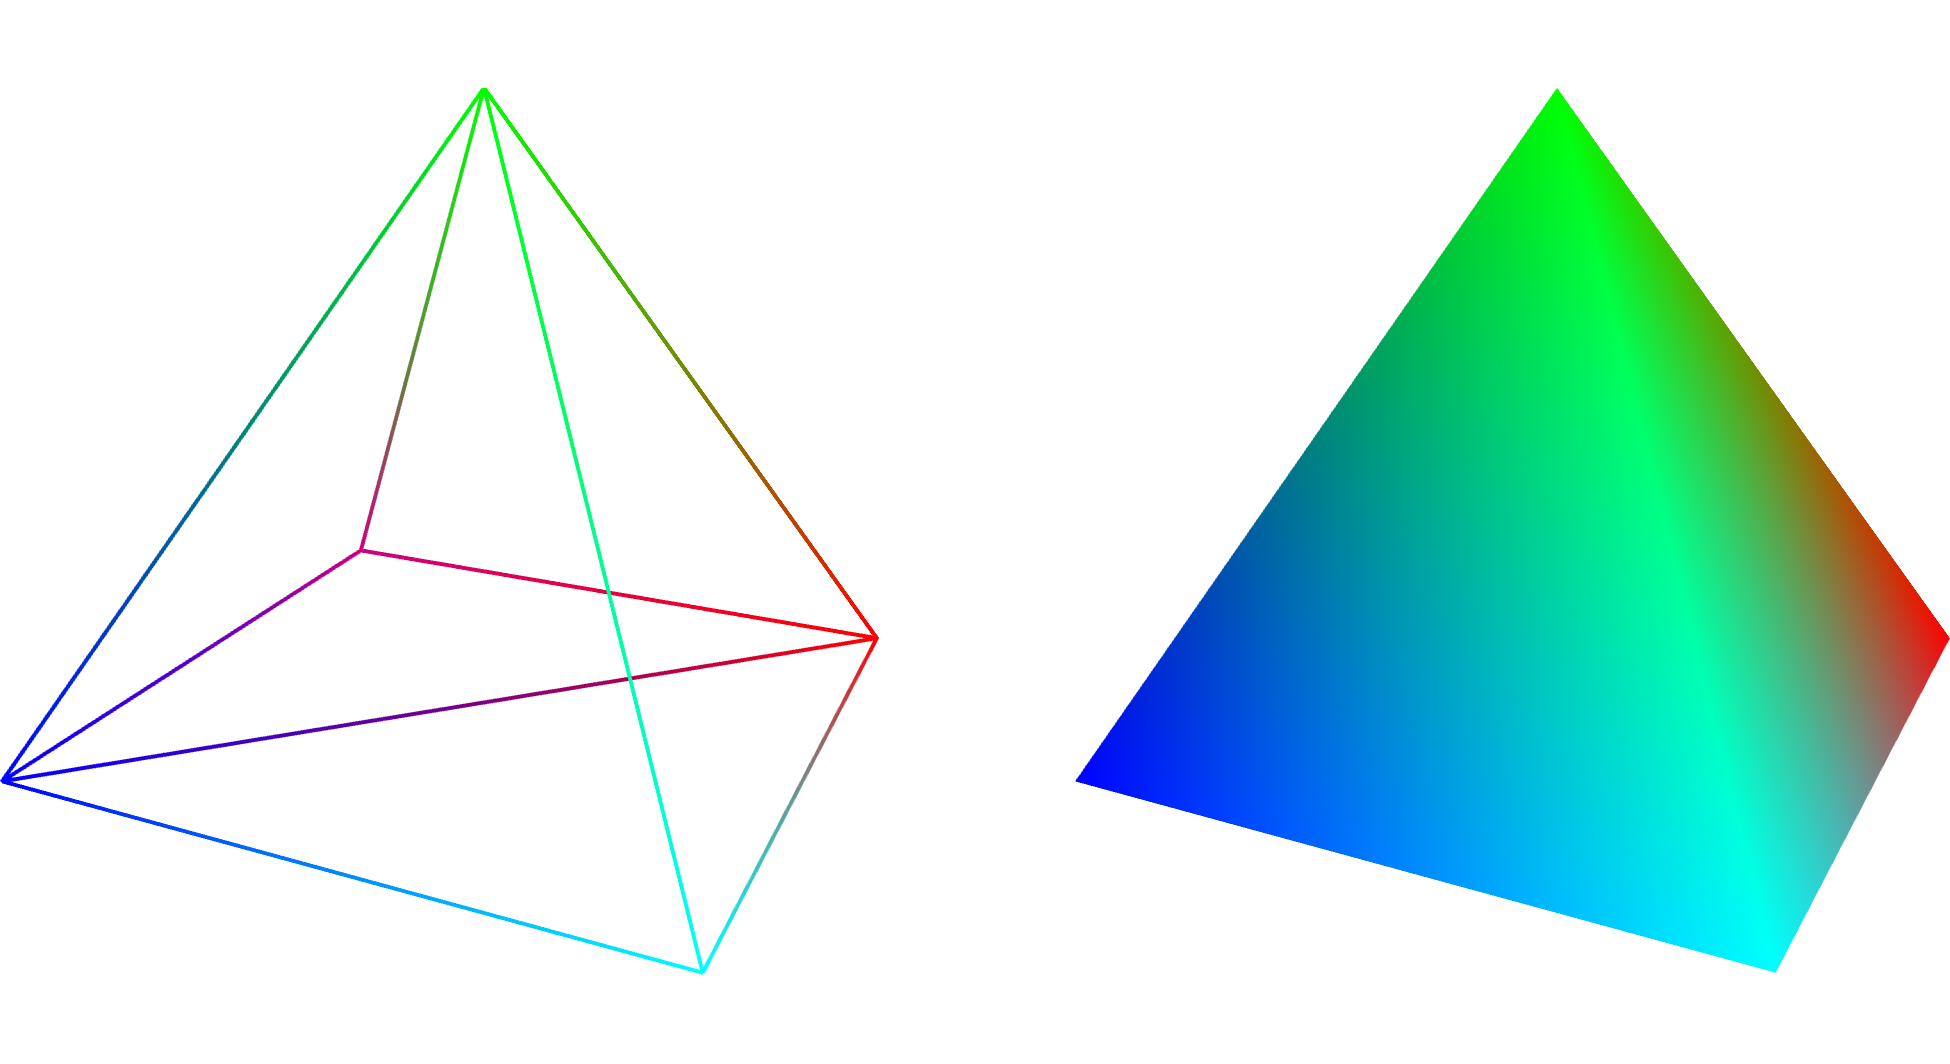
\includegraphics[width=0.6\textwidth]{kap4/webgl/figures/pyramid_views.png}
	\caption{Verschiedene Ansichten der Beispiel-Anwendung.}
	\label{FIG:WEBGL_EXAMPLE_VIEWS}
\end{figure}

Zusätzlich zu den vorherigen Einstellungmöglichkeiten bezüglich Projektionsart und Animation kann die Ansicht nun wie in Abbildung \ref{FIG:WEBGL_EXAMPLE_VIEWS} dargestellt zwischen dem Drahtgittermodell der Figur und gefüllten Flächen umgeschaltet werden.

Der Programmablauf kann wie folgt skizziert werden:

\begin{enumerate}[noitemsep]
	\item Initialisierung des WebGL-Kontexts und Setzen grundlegender Einstellungen.
	\item Erstellung des Fragment- und Vertex-Shaders.
	\item Erstellung der \emph{Buffer Objects} und Schreiben der Vertex-Attribute.
	\item Optional: Animation der geometrischen Figur.
	\item Berechnung und Darstellung des Einzelbilds (Rendering).
\end{enumerate}

Als Einstiegspunkt der Anwendung dient die \texttt{main}-Funktion, welche obigen Ablauf durch mehrere Funktionsaufrufe abbildet. Der Sinn und Zweck der verschiedenen Funktionen wird in den folgenden Abschnitten erklärt.

\smallskip
\begin{listing}[!htb]
\jsginput[firstline=15, lastline=35, firstnumber=15]{kap4/webgl/example/main.js}
\caption{Main-Methode.}
\label{LISTING:WEBGL_EXAMPLE_MAIN}
\end{listing}

\subsubsection{Initialisierung des WebGL-Kontexts}

In den Zeilen 16 bis 25 (vgl. Listing \ref{LISTING:WEBGL_EXAMPLE_MAIN}) wird zunächst der WebGL-Kontext mittels des Canvas-DOM-Elements abgefragt und in der Variable \texttt{gl} gespeichert. In manchen Browser-""Implementierungen von WebGL trägt der Kontext noch die Bezeichnung \texttt{ex"-per"-imen"-tal-""webgl}, welche auf die noch experimentelle Unterstützung der Technologie hinweist. Um eine möglichst breite Browserunterstützung zu erzielen, wird daher auch auf diesen Bezeichner hin geprüft. Die Option \texttt{antialias} aktiviert das Anti-Aliasing und sorgt so für eine glattere Kantendarstellung.

Sofern die Schnittstelle erfolgreich initialisiert werden konnte, werden die weiteren Funktionen \texttt{initGl}, \texttt{initShaders}, \texttt{initBuffers}, und \texttt{tick} aufgerufen. Die \texttt{initGl}-Routine (vgl. Listing \ref{LISTING:WEBGL_EXAMPLE_INIT_GL}) legt einige grundsätzliche Einstellungen fest:
Als erstes wird der Tiefenpuffer aktiviert (\emph{Z-Buffering}). Hierdurch werden Gegenstände, die sich auf der Z-Achse hinter einem weiteren Objekt befinden, im Rasterisierungsschritt verdeckt, so wie es der natürlichen Wahrnehmung entspricht. Weiterhin wird die Breite der zu zeichnenden Linien und die Hintergrundfarbe der Projektionsfläche festgelegt. Der Funktionsaufruf \texttt{gl.clear} in Zeile 50 bewirkt das Zurücksetzen des Farb- und Tiefenpuffers und führt so zu einer komplett weißen, leeren Zeichenfläche.

\smallskip
\begin{listing}[!h]
\jsgginput[firstline=47, lastline=51, firstnumber=47]{kap4/webgl/example/main.js}
\caption{Initialisierung des WebGL-Kontexts.}
\label{LISTING:WEBGL_EXAMPLE_INIT_GL}
\end{listing}

\vspace{1ex}

\begin{listing}[!h]
\jsginput[firstline=62, lastline=75, firstnumber=62]{kap4/webgl/example/main.js}
\caption{Berechnung der Sicht-Projektions-Matrix.}
\label{LISTING:WEBGL_EXAMPLE_CALC_VP_MATRIX}
\end{listing}

Zur Berechnung der Sicht- und Projektionsmatrix wird die Hilfsfunktion \texttt{calc"-View"-Proj"-Matrix} aufgerufen (vgl. Listing \ref{LISTING:WEBGL_EXAMPLE_CALC_VP_MATRIX}). Innerhalb dieser Methode wird zunächst die Sichtmatrix durch Aufruf der \texttt{mat4.lookAt}-Funktion der \emph{glMatrix}"=Bibliothek erstellt. Hierbei fließen Augpunkt, das Zentrum der Beobachtung (\emph{Look-at-Punkt}) und Oben-Vektor ein. Je nach aktueller Einstellung wird anschließend entweder eine orthogonale Projektionsmatrix durch Angabe der Ausdehnung des Sichtvolumens erstellt oder die Projektionsmatrix für eine perspektivische Darstellung erzeugt. In letzerem Fall wird ebenso die Abmessung des \emph{Frustums} und die Distanz der \emph{Front-} und \emph{Backplane} als Parameter benötigt.

Die Berechnung dieses Matrizenprodukts dient der Einsparung von Rechenzeit. Während sich die Modellmatrix durch die Animation kontinuierlich ändert, bleibt die Sicht-Projektions-Matrix größtenteils gleich.

\subsubsection{Initialisierung der Shader}

Im nächsten Schritt werden die im HTML-Dokument eingebetten Shader durch die Hilfsmethode \texttt{getShader} eingelesen und verarbeitet. Hierbei wird je nach Typ ein entsprechendes Shader-Objekt erstellt, der Quelltext aus den Script-Tags eingefügt und dieser schließlich kompiliert. Listing \ref{LISTING:WEBGL_EXAMPLE_GET_SHADER} zeigt den relevanten Abschnitt der Funktion.

\smallskip
\begin{listing}[!htb]
\jsgginput[firstline=110, lastline=120, firstnumber=110,]{kap4/webgl/example/main.js}
\caption{Auslesen der Shader-Quelltexte.}
\label{LISTING:WEBGL_EXAMPLE_GET_SHADER}
\end{listing}

Anschließend wird das Shader-Programm-Objekt erstellt und der kompilierte Shader-Code angehängt. Durch Aufruf der \texttt{linkProgram}"=Methode wird das Programm zu einer für die GPU verarbeitbaren Binärdatei gebunden (\emph{Linking}). Sofern hierbei kein Fehler aufgetreten ist, wird WebGL angewiesen, die so gepackten Shader beim Rendering-Vorgang für die Berechnung der Darstellung zu verwenden (vgl. Listing \ref{LISTING:WEBGL_EXAMPLE_INIT_SHADERS}, Zeile 92). Zuletzt wird die Speicherposition der Uniform-Variable \texttt{uMVPMatrix} innerhalb des Vertex-Shaders abgefragt. Dies ist notwendig, um deren Wert während der späteren Animation aktualisieren zu können. Eine Uniform-Variable zeichnet sich dadurch aus, dass sie sowohl im Vertex- als auch im Fragment-Shader zur Verfügung steht \autocite{Matsuda:2013}.

\smallskip
\begin{listing}[!htb]
\jsginput[firstline=80, lastline=95, firstnumber=80]{kap4/webgl/example/main.js}
\caption{Erstellung und Binden des Shader-Programms.}
\label{LISTING:WEBGL_EXAMPLE_INIT_SHADERS}
\end{listing}

\subsubsection{Erstellung und Schreiben der Daten-Puffer}

Um den Shadern innerhalb von WebGL Daten zu übergeben, werden sogenannte \emph{Vertex Buffer Objects} (VBO) verwendet. Ein solches Buffer Object stellt einen Speicherbereich innerhalb der GPU dar, welcher verschiedene Vertex-Attribute aufnimmt. In der Beispiel-Anwendung beschreiben drei verschiedene solcher Puffer die Geometrie und Farben der Pyramide.
Bei der Definition dieser Rohdaten kommen sogenannte \emph{TypedArrays} zum Einsatz. Diese speziellen Arrays bieten aufgrund ihrer starken Typenbindung bei großen Datenmengen bessere Performance gegenüber konventiellen JavaScript-Feldern, da der Zugriff entsprechend optimiert werden kann \autocite{JS_TYPED_ARRAYS}.

\smallskip
\begin{listing}[!h]
\jsgginput[firstline=134, lastline=149, firstnumber=134]{kap4/webgl/example/main.js}
\caption{Definition der Vertices und Seiten der Pyramide.}
\label{LISTING:WEBGL_EXAMPLE_INIT_BUFFERS_ARRAYS}
\end{listing}

Im ersten Puffer werden die fünf Eckpunkte (\emph{Vertices}) der Figur durch ihre kartesischen Koordinaten im Raum angegeben (vgl. Listing \ref{LISTING:WEBGL_EXAMPLE_INIT_BUFFERS_ARRAYS}). Der zweite Puffer legt die Seiten der Figur fest. Hierfür werden je drei der zuvor definierten Punkte anhand ihrer Indices zu einem Dreieck verbunden. Zu beachten ist, dass die Nummerierung der Indices bei 0 beginnt. Die Reihenfolge der Punkte ist aufgrund des \emph{Backface Culling} wichtig. Dieses Verfahren dient der Verbesserung der Darstellungseffizienz, indem nur die durch den Normalenvektor definierte Vorderseite von Dreiecken gezeichnet wird. Das letzte hier nicht gezeigte Array spezifiziert schließlich die Farben der Pyramide, indem die RGB-Werte den fünf Punkten ihrer Reihenfolge entsprechend zugeordnet werden. Die Farbkanäle werden in WebGL analog zu X3D im Zahlenintervall $[0,1]$ angegeben.

\smallskip
\begin{figure}[!htb]
	\centering
	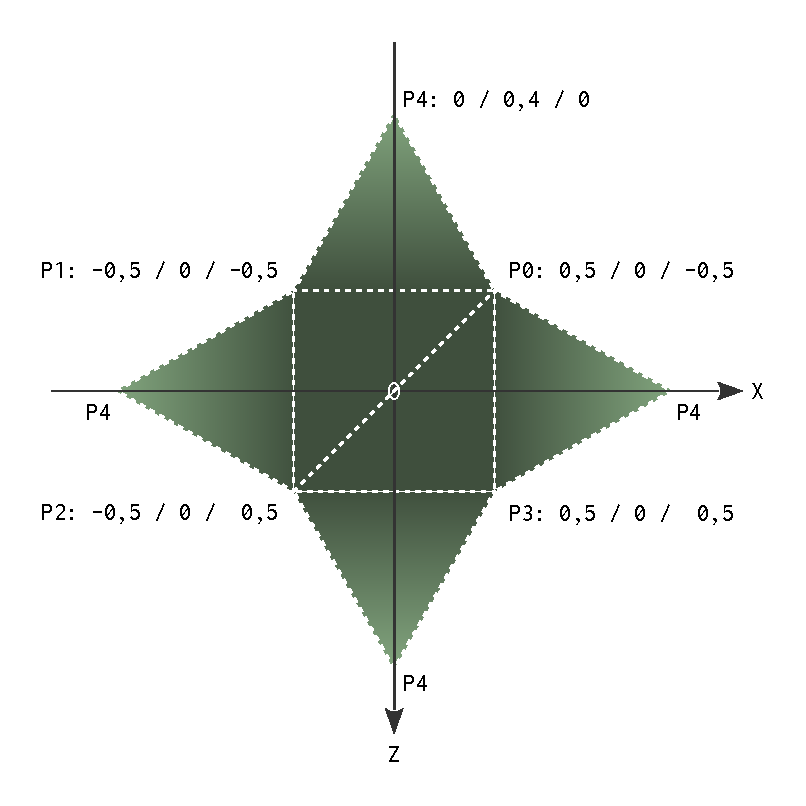
\includegraphics[width=0.5\textwidth]{kap4/webgl/figures/pyramid_sketch-crop.pdf}
	\caption{Topologische Struktur der Pyramide.}
	\label{FIG:WEBGL_EXAMPLE_PYRAMID_SKETCH}
\end{figure}

Abbildung \ref{FIG:WEBGL_EXAMPLE_PYRAMID_SKETCH} veranschaulicht den topologischen Aufbau der Pyramide, indem deren Geometrie innerhalb der XZ-Ebene aufgespannt wurde. Dies erleichtert die Nachvollziehbarkeit der obigen Indices-Zuweisung.

\smallskip
\begin{listing}[!htb]
\begin{minted}[linenos, fontsize=\footnotesize, tabsize=4, baselinestretch=1,firstnumber=168]{javascript}
buffer = gl.createBuffer();
gl.bindBuffer(gl.ARRAY_BUFFER, buffer);
gl.bufferData(gl.ARRAY_BUFFER, vertices, gl.STATIC_DRAW);

FSIZE = vertices.BYTES_PER_ELEMENT;
attribute = gl.getAttribLocation(gl.program, 'aPosition');
gl.vertexAttribPointer(attribute, 3, gl.FLOAT, false, FSIZE * 3, 0);
gl.enableVertexAttribArray(attribute);
\end{minted}
\caption{Schreiben der Puffer-Daten}
\label{LISTING:WEBGL_BINDING_OF_BUFFERS}
\end{listing}

Für das Schreiben der Puffer in den Speicher der GPU sind mehrere Schritte notwendig: Zunächst muss ein Buffer-Objekt durch die WebGL-API erstellt werden. Anschließend wird dieses durch die \texttt{bindBuffer}-Methode als derzeitiger Arbeitspuffer ausgewählt. Die eigentlichen Daten -- hier das Array mit den Vertices -- können dann durch Aufruf von \texttt{bufferData} geschrieben werden (Zeile 168 ff.).
Im nächsten Schritt wird die Speicherposition der Shader-Variable \texttt{aPosition} abgefragt, um diese mit dem Daten-Puffer zu verknüpfen (Zeile 173). Dies wird durch die Funktion \texttt{vertexAttribPointer} realisiert. Dabei gibt deren fünfter Parameter an wie viele Bytes zwischen Beginn und Ende der Definition einer Seite der Pyramide im Vertex-Buffer liegen. Da je drei Eckpunkte eine Seite definieren, wird dieser Wert mit der Länge eines Einzelelements (\texttt{FSIZE}) multipliziert. Mit dem Aufruf von \texttt{enableVertexAttribArray} wird das Vertex-Attribut schließlich aktiviert. Nachdem der Farb- und Indexpuffer auf die selbe Weise an die Grafikhardware gereicht wurden, kann das eigentliche Rendering der Figur beginnen.

\subsubsection{Animation der geometrischen Figur}

Die Funktion \texttt{tick}, welche initial in der \texttt{main}-Routine aufgerufen wurde, ist für die Animation und Berechnung des Einzelbilds verantwortlich. Sofern die Bewegung der Pyramide mittels des Kontrollkästchens aktiviert ist, wird die Animation gestartet (vgl. Listing \ref{LISTING:WEBGL_EXAMPLE_TICK}, Zeile 191). Im Anschluss wird die Rendering-Funktion aufgerufen und die erneute Ausführung von \texttt{tick} durch die \texttt{requestAnimationFrame}-Methode angefordert (Zeile 195 f.).
\texttt{requestAnimationFrame} stellt einen vom Browser bereitgestellte Mechanismus zur Optimierung von JavaScript-Animationen dar \autocite{OPERA_REQUEST_ANIMATION_FRAME}. Der nächste Animationsschritt wird hierbei vom Webbrowser unter Berücksichtigung der aktuellen CPU-Last eingeplant, anstatt diesen nach einem fixen Zeitinkrement auszuführen. Hierdurch wird eine flüssigere Animation erzielt. Ein weiterer Vorteil ist die Einsparung von Rechenzeit und Akkuverbrauch, da die Animationsschleife nur dann ausgeführt wird, wenn der entsprechende Browser-Tab aktiv ist. Dies ist insbesondere bei Mobilgeräten ein wichtiger Aspekt.

\smallskip
\begin{listing}[!htb]
\jsginput[firstline=189, lastline=197, firstnumber=189]{kap4/webgl/example/main.js}
\caption{Einzeliteration der Animation.}
\label{LISTING:WEBGL_EXAMPLE_TICK}
\end{listing}

Die eigentliche Animation der Rotation um die Y-Achse erfolgt durch die Funktion \texttt{animate}. Da das Zeitintervall zwischen zwei Aufrufen der Animations-Methode variieren kann, kann eine ungleichmäßige Bewegung entstehen, sofern stets das gleiche Inkrement zum Rotationswinkel hinzuaddiert wird. Unter Berücksichtigung des Zeitintervalls zwischen zwei Iterationen kann dieses Defizit leicht behoben werden, indem der ermittelte Delta-Wert in die Berechnung dieses Inkrements einfließt (vgl. Listing \ref{LISTING:WEBGL_EXAMPLE_ANIMATE}, Zeile 215). Der Modulo-Operator sichert den Wertebereich von $[0, 360]$ Grad.

\smallskip
\begin{listing}[!htb]
\jsginput[firstline=202, lastline=212, firstnumber=202]{kap4/webgl/example/main.js}
\caption{Animation der Rotation.}
\label{LISTING:WEBGL_EXAMPLE_ANIMATE}
\end{listing}

Da die Grundfläche der Pyramide genau mittig innerhalb der XZ-Ebene liegt und deren Normale auf die Spitze so genau mit der Y-Achse zusammenfällt, ist die Berechnung der Rotation hier sehr einfach. Die Modellmatrix muss lediglich auf die Rotationsmatrix um die Y-Achse für diesen Winkel gesetzt werden. Dies wird durch Aufruf der \texttt{mat4.rotateY}-Funktion aus der \emph{glMatrix}-Bibliothek in Zeile 211 erzielt.

\subsubsection{Rendering des Einzelbilds}

Schließlich kann der Rendering-Prozess der virtuellen Pyramidendarstellung angestoßen werden. Hierfür wird zunächst die MVP-Matrix durch Multiplikation der aktuellen Modellmatrix mit der Sicht-Projektionsmatrix berechnet (vgl. Listing \ref{LISTING:WEBGL_EXAMPLE_RENDER} Zeile 219). Anschließend wird das Ergebnis mittels Aufruf der \texttt{uniformMatrix4fv}-Methode an den Vertex-Shader übergeben.

\smallskip
\begin{listing}[!htb]
\jsginput[firstline=218, lastline=225, firstnumber=218]{kap4/webgl/example/main.js}
\caption{Rendering der Darstellung.}
\label{LISTING:WEBGL_EXAMPLE_RENDER}
\end{listing}

\begin{listing}[!htb]
\begin{jscode}
void main(void) {
	gl_Position = uMVPMatrix * a_Position;
	v_Color = a_Color;
}
\end{jscode}
\caption{Hauptfunktion des Vertex-Shaders.}
\label{LISTING:WEBGL_VERTEX_SHADER}
\end{listing}

Der Vertex-Shader, gezeigt in Listing \ref{LISTING:WEBGL_VERTEX_SHADER}, ist äußerst simpel gehalten und entspricht dem gezeigten Verfahren bei Betrachtung der Standard-Grafikpipeline in Abschnitt \ref{SEC:STANDARD_GRAPHICS_PIPELINE}. Die endgültige Position jedes Vertex wird durch Multiplikation der Koordinaten mit der MVP-Matrix realisiert (vgl. Listing \ref{LISTING:WEBGL_VERTEX_SHADER}, Zeile 3). Der Fragment-Shader ist ebenfalls einfach gehalten. Den einzelnen Fragmenten wird lediglich die zuvor spezifzierte Farbe zugewiesen. Durch die standardmäßige Interpolation der Farben der Eckpunkte bei OpenGL ergeben sich die Farbverläufe auf den Seiten der Figur.

Nachdem der Farb- und der Tiefenpuffer geleert wurde, kann das Bild schließlich mit der gewählten Methode gezeichnet und in den Framebuffer geschrieben werden (vgl. Listing \ref{LISTING:WEBGL_EXAMPLE_RENDER}, Zeile 222 ff.).

\subsection{Three.js als Vertreter eines WebGL-Frameworks}

Wie das vorherige Beispiel zeigt, ist aufgrund des niedrigen Abstraktionsniveaus der WebGL-API im Vergleich zu X3D ein sehr viel höherer Aufwand notwendig, um selbst einfachste dreidimensionale Szenen darzustellen. Da sich jedoch viele Teile des Programmes wie beispielsweise die Abfrage des WebGL-Kontexts oder die Initialisierung der Shader bei jeder WebGL-basierten Anwendung wiederholen, ist eine Generalisierung dieser immer wieder benötigten Funktionalität auf höherer Ebene naheliegend.

Innerhalb der letzten Jahre entstanden so zahlreiche, zum Teil sehr umfangreiche und ausgereifte Frameworks, welche die Umsetzung grafisch anspruchsvoller 3D-""Anwendungen erheblich erleichtern. So können Basiselemente wie Geometrien, Texturen, Lichtquellen, Kameras et cetera mittels weniger Funktionsaufrufe komfortabel erstellt und einem Szenengraph hinzugefügt werden.

Eine Methode zur groben Beurteilung der Popularität von Software stellt die Anzahl von Favorisierungen (Sterne) auf dem Portal \emph{GitHub} dar \autocite{Evans201443}. GitHub ist ein Hosting-Dienst für Repositories der Versionsverwaltung Git, welcher insbesondere bei Open-Source-Projekten beliebt ist. Das Framework \emph{Three.js} des spanischen Webentwicklers Ricardo Cabello\footnote{Besser bekannt als \emph{Mr.doob}.} liegt hierbei mit einem Wert von 15.558 Sternen weit vor dem hinsichtlich dieses Kriteriums zweitpopulärsten Systems \emph{PhiloGL}, welches mit 567 Stimmen lediglich einen Bruchteil dieses Werts verbuchen kann \autocite{SOFTWARE_GITHUB_THREEJS} \autocite{SOFTWARE_GITHUB_PHILOGL}.
Zusätzlich zu der generellen Vereinfachung bei der Erstellung einer 3D-Szene bietet Three.js ähnlich zu X3DOM verschiedene Rendering-Backends, die als Fallback-Lösungen dienen können. Neben WebGL kann die Darstellung auch innerhalb eines 2D-Canvas, durch SVG oder durch CSS3-Transformationen erfolgen. Aufgrund der deutlich schlechteren Performance dieser Techniken und der Fokusierung dieser Arbeit auf WebGL und X3D, werden diese Technologien jedoch nicht näher betrachtet.

Sämtliche weiteren Untersuchungen von WebGL innerhalb des Evaluationsteils werden aufgrund der genannten Vorteile eines abstrahierten WebGL-Frameworks auf Basis von Three.js realisiert.
